\begin{frame}
	\frametitle{Diagonalisierung}
	\framesubtitle{Was verstehen wir darunter?}
	
	
	


	\begin{figure}
			\begin{minipage}{0.8\linewidth}
				\begin{itemize}[<+->]
					\item Cantors Diagonalargument zur Überabzählbarkeit von $ \mathbb{R}$
					\item Unentscheidbarkeit des Halteproblems
					\item informell: Konstruktion eines Elements, das sich von jedem anderen Element unterscheidet
					\item Diagonalisierung nicht immer "schön" zu sehen
				\end{itemize}
			\end{minipage}
			\begin{minipage}{0.1\linewidth}
					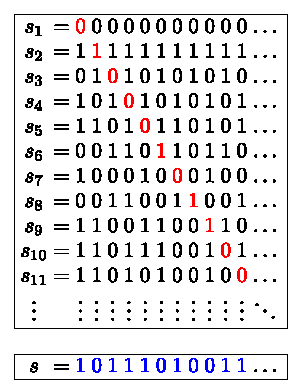
\includegraphics[scale = 0.4]{images/Diagonal_argument_svg.pdf}%
			\end{minipage}
		\end{figure}
	
\end{frame}
\begin{frame}
	\frametitle{Diagonalisierung}
	\framesubtitle{Was verstehen wir darunter?}
	\begin{KITinfoblock}{Was ist Diagonalisierung} {
			Als Diagonalisierung wird (hier) ein Beweis bezeichnet, der nur auf den beiden folgenden
			Eigenschaften von TM aufbaut.
			
			\begin{enumerate}
				\item<2-> Die Existenz einer Repräsentation von TM durch Zeichenketten (Gödelnummer)
				\item<3-> Die Fähigkeit eine andere TM mit geringem zusätzlichen Zeit- oder Platzbedarf zu simulieren (Universelle TM)
			\end{enumerate}		
		}
	\end{KITinfoblock}
	
\end{frame}